\begin{exercise}
      {ID-c632feb239d82bb8318754dcb73efe693d5d9aef}
      {Bilddiagonale}
  \ifproblem\problem
    Bildschirme von Fernsehgeräten gibt es in zwei unterschiedlichen Formaten.
    Das Verhältnis von Breite zu Höhe beträgt bei älteren Geräten 4:3, bei
    neuen 16:9. Die Bildschirmgröße wird in der Regel mit der Länge der
    Bilddiagonalen angegeben.
    \begin{enumerate}[a)]
      \item Berechne Höhe und Breite von Bildschirmen mit den Bilddiagonalen
            \sicm{69} und \sicm{89} bei einem 4:3-Format. Um wie viel cm\textsuperscript{2}
            unterscheiden sich die beiden Bildschirmflächen?
      \item Wenn ein Film im 16:9-Format auf einem Bildschirm im 4:3-Format gezeigt
            wird, sieht man oben und unten schwarze Streifen. Wie viel Prozent der
            Bildfläche wird von dem Film eingenommen?
      \item \xxa{} hat einen \num{89}er-Bildschirm im Format 4:3. Beim Format 16:9 bleiben
            bei herkömmlichen Sendungen rechts und links Streifen, falls die Höhe
            voll ausgenutzt wird. \xxa{} möchte einen neuen Fernseher im Format
            16:9 kaufen. Dabei soll eine herkömmliche Sendung dieselbe Größe haben
            wie bisher. Welche Bildschirmdiagonale muss \xxa{} kaufen?
    \end{enumerate}
  \fi
  %\ifoutline\outline
  %\fi
  \ifoutcome\outcome
    \begin{enumerate}[a)]
      \item Ein Bildschirm im Format 4:3 ist \sicm{55.2} breit und \sicm{41.4} hoch,
            wenn seine Diagonale \sicm{69} lang ist, und mit einer Diagonalen von
            \sicm{89} besitzt er eine Breite vom \sicm{71.2} und eine Höhe von
            \sicm{53.4}.\par
            Die Bildschirmflächen unterscheiden sich um \sicmm{1516.8}.
      \item Bei gleicher Breite ist die Fläche des 16:9 Bildschirms \pc{25}
            kleiner als die Fläche des Bildschirms im 4:3-Format:\par
            \begin{minipage}{6.25cm}
              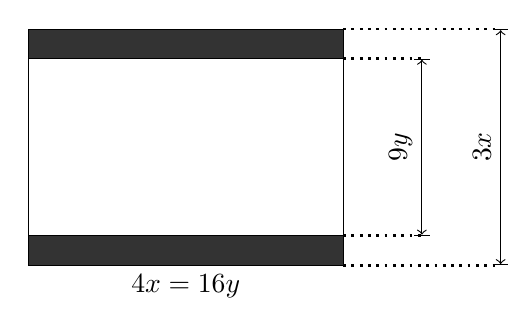
\begin{tikzpicture}
                \begin{scope}[xshift=-2cm, yshift=-1.5cm]
                  \filldraw[fill=black!80!white, draw=black]
                    (0, 0) rectangle (4, 3);
                    \node[below] at (2, 0) {$4x=16y$};
                  \draw[style=dotted, line width=1pt] (4, 3) -- +(2, 0);
                  \draw[style=dotted, line width=1pt] (4, 0) -- +(2, 0);
                \end{scope}
                \begin{scope}[xshift=-2cm, yshift=-1.125cm]
                  \filldraw[fill=white, draw=black]
                    (0, 0) rectangle (4, 2.25);
                  \draw[style=dotted, line width=1pt] (4, 2.25) -- +(1, 0);
                  \draw[style=dotted, line width=1pt] (4, 0) -- +(1, 0);
                \end{scope}
                \draw[|<->|] (3, -1.125) -- node[above, rotate=90]{$9y$} (3, 1.125);
                \draw[|<->|] (4, -1.5) -- node[above, rotate=90]{$3x$} (4, 1.5);
              \end{tikzpicture}%
            \end{minipage}%
            \hfill
            \begin{minipage}{20em}
              \setlength{\abovedisplayskip}{0pt}%
              \begin{equation*}
                4x=16y
                \quad\Rightarrow\quad
                y=\frac{x}{4}
                \quad\Rightarrow\quad
                9y=\frac{9x}{4}
              \end{equation*}
              \par
              \begin{equation*}
                \frac{16y\cdot9y}{4x\cdot3x}
                =
                \frac{4x\cdot\frac{9x}{4}}{4x\cdot3x}
                =
                \frac{3}{4}
                =
                \pc{75}
              \end{equation*}
            \end{minipage}\par
            Das Bild eines 16:9 Films nimmt also nur \pc{75} der
            Flache eines 4:3 Bildschirms ein.
      \item Um auf dem neuen 16:9 Bildschirm einen Film im 4:3-Format in derselben Größe
            ansehen zu können wie auf einem 4:3 Bildschirm mit \sicm{89} Diagonalenlänge,
            braucht der neue Bildschirm eine Diagonale von \sicm{108.9}.
    \end{enumerate}
  \fi
\end{exercise}
